\pdfminorversion=4
\documentclass{beamer}
\usepackage[T1]{fontenc}
\usepackage[ngerman]{babel}
\usepackage[utf8]{inputenc}
\usepackage[babel,german=quotes]{csquotes}
\usepackage{amsmath,amsfonts,amssymb}
\usepackage{hyperref}
\usepackage{lmodern}
\usepackage{microtype}

\usetheme{fau-4-3}

\usepackage[sort&compress,comma,super,square]{natbib}
%\bibliographystyle{apalike} % Or your specific bibliographystyle
\bibliographystyle{unsrtdin}
%\bibliographystyle{gerplain}

\newcommand{\todo}[1]{\textbf{\color{red}{TODO: #1}}}


\title{cowbusconfig – Ansatz zur dezentralen Konfiguration von Gebäudeautomation}
\author[P. Kanzler, M. Zapf]{Patrick\,Kanzler \and Michael\,Zapf}
\date{23.09.2015}


\begin{document}
\frame{\titlepage}

%\section{cowbusconfig – Ansatz zur dezentralen Konfiguration von Gebaueudeautomation}
\begin{frame}
	\frametitle{Der Traum von der schönen neuen Welt}
	
	\begin{itemize}
		\item \todo{schön darstellen, vielleicht mit Bildern, momentan nur Stichpunkte}
		\item Haus der Zukunft
		\item Beleuchtung folgt intelligent durch das Haus
		\item Haus weiß anhand des Kalenders und Heuristik, wann welcher Raum zu heizen ist
		\item ... andere schicke Beispiele für Heimautomatisierung
	\end{itemize}
\end{frame}

\begin{frame}
	\frametitle{Ausgeträumt!}
	
	\begin{itemize}
		\item Der Knotenkontroller der Kaffemaschine spricht eine schlechte Implementierung des\
		Automatisierunsgprotokolls und bringt damit den zentralen Server zum abstürzen
		\item Es wird unerträglich warm, die Heizung bleibt auf dem letzten Wert hängen
		\item Lüften geht nicht, weil die Rollos nicht hoch gehen.
		\item Nichteinmal das Licht geht an. Hätte ich vielleicht doch die starre Verdrahtung drin gelassen?
	\end{itemize}
\end{frame}

\begin{frame}
    \frametitle{Ziele und Ideen}

    \begin{itemize}
        \item dezentrale Organisation, um single-point-of-failure zu umgehen
        \item Trotzdem: komfortable Konfiguration, nicht jeden Knoten anfassen müssen
        \item OpenSource, (??? anpassbar an eigene Bedürfnisse, dennoch auch \enquote{out of the box} funktionsfähig ???)
        \item Verwendung einer fertigen Betriebssystemplattform, um Entwicklungsaufwand zu sparen und Portierbarkeit zu erhöhen
        \item Auftrennung in \enquote{dumme} Sensoren und \enquote{intelligente} Aktoren
    \end{itemize}
\end{frame}

\begin{frame}
    \frametitle{Regeln}

    \begin{itemize}
        \item 
        \item
        \item
        \item
        \item
        \item
    \end{itemize}
\end{frame}

\begin{frame}
    \frametitle{Konfigurationsnachrichten}

    \begin{itemize}
        \item
        \item
        \item
        \item
        \item
    \end{itemize}
\end{frame}

\begin{frame}
    \frametitle{Demo}
\end{frame}

\section{Q\&A}

\section{Vielen Dank für Ihre Aufmerksamkeit!}

%\begin{frame}[plain]
%    \center
%    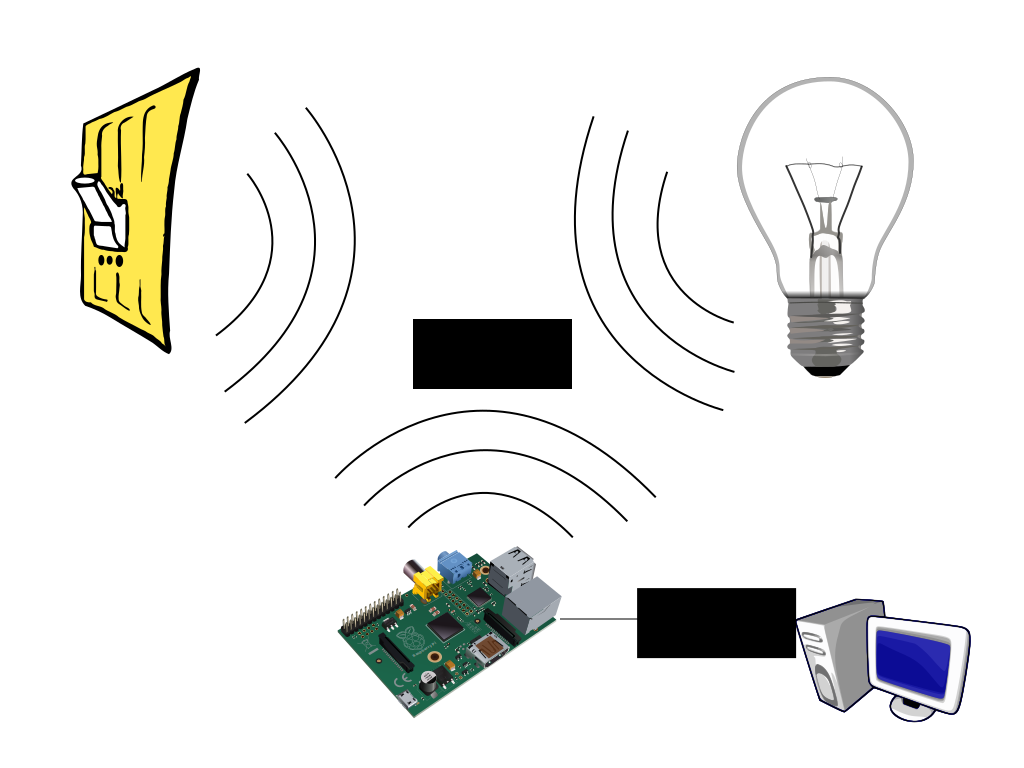
\includegraphics[scale=0.4]{img/system}
%\end{frame}


%\nocite*
%\bibliography{2015-09-cowconfig}{}

\end{document}

